
\begin{figure*}[t]
    \centering
    \begin{subfigure}{0.35\textwidth}
      \centering
      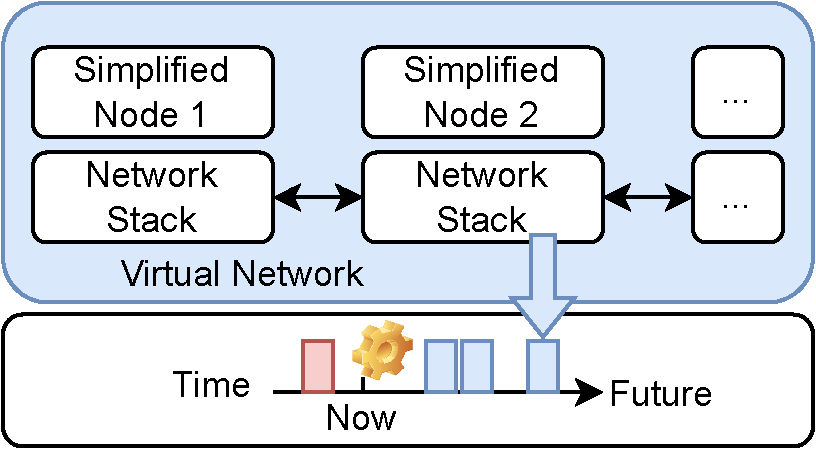
\includegraphics[width=\linewidth]{Figs/DES.drawio.pdf}
      \caption{Conventional DES}
      \label{fig:des}
    \end{subfigure}%
    \hspace{2em}
    \begin{subfigure}{0.35\textwidth}
      \centering
      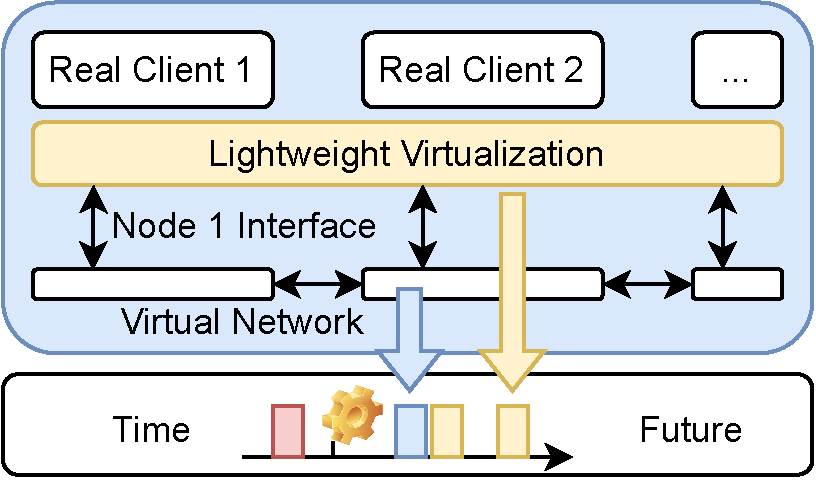
\includegraphics[width=\linewidth]{Figs/DES2.drawio.pdf}
      \caption{DES with real-client execution}
      \label{fig:des-shadow}
    \end{subfigure}
    \vspace{-0.5em}
    \caption{Comparison of conventional discrete-event simulation (DES) and DES with real applications. \textbf{Subfigure (a)} Conventional DES: a network simulator translates network traffic and an abstract node model into discrete events scheduled on a unified timeline. \textbf{Subfigure (b)} DES with real-client execution: the simulator retains the same event-driven network core, but replaces the abstract node model with a lightweight virtualization layer that executes real client applications. Application and network events coexist on a single time axis under a shared simulation clock.}
    \label{fig:DESs}
\end{figure*}
  
\section{Time-Decoupled Testnet Framework}
\label{sec:edt}
  
This section presents our \emph{time-decoupled testnet framework}, which executes real blockchain client software atop an event-driven execution substrate while exposing protocol time as an explicit control surface. The key goal is not merely to run a testnet faster, but to make logical time \emph{controllable} for strongly time-controlled consensus protocols without sacrificing real-client execution.
  
\subsection{Key Idea: Controllable Time for Real-Client}
\label{subsec:edt-keyidea}
  
For strongly time-controlled consensus protocols, the central testing bottleneck is not merely insufficient input generation, but the inability to control \emph{when protocol time advances}. In a conventional real-time testnet, testers can perturb messages and network conditions, but they cannot decouple protocol progress from wall-clock time. As a result, large fractions of execution are spent waiting for the next slot/epoch boundary, and time-gated consensus logic remains sparsely exercised.
  
Simulators handle this situation well because they already treat time as part of the execution model: event-driven simulation naturally advances from one causally relevant event to the next, skipping empty intervals and providing strong control over time and schedules. However, simulators usually achieve this at the cost of re-implementing protocol logic in simplified models, which weakens implementation fidelity and limits their ability to expose bugs in real clients.
  
Testnets occupy the opposite point in the design space. They execute real, unmodified clients and therefore preserve implementation fidelity, but for strongly time-controlled protocols they inherit substantial temporal redundancy: protocol progress remains tied to wall-clock time, and testing cannot systematically control or compress the idle intervals between meaningful protocol transitions.
  
Our key idea is therefore to combine \emph{real-client execution} with \emph{controllable logical time}. Rather than requiring the framework to understand protocol-specific concepts such as slots or epochs explicitly, we make logical time itself controllable: the execution substrate can pause, resume, replay, and advance time deterministically, while real clients continue to run unmodified. For strongly time-controlled protocols, this is already sufficient to reach and re-exercise timing-sensitive regions of execution efficiently.
  
Concretely, the framework runs real client binaries inside virtual hosts on top of an event-driven substrate (Figure~\ref{fig:DESs}(b)). Idle waits become pending events on a unified logical timeline, and execution advances directly to the next causally ready event rather than waiting for wall-clock time to pass. The result is a time-decoupled testnet that preserves real-client execution while exposing protocol-time progression as a testing primitive.
  
\subsection{Principles}
\label{sec:design_principles}
  
Making protocol time controllable is useful only if the resulting framework remains meaningful for testing. In particular, controllable time must not come at the cost of changing protocol semantics, breaking reproducibility, or abandoning real-client execution. We therefore structure the framework around four design requirements.

\smallskip
\noindent\textbf{P1: Semantic equivalence of protocol time.}
Controlling time must not change the \emph{meaning} of time in the protocol. Event-driven execution must preserve the causal semantics induced by the protocol's logical clock and time-dependent rules.
In particular, advancing logical time must not skip or reorder mandatory time-triggered transitions, and it must preserve the intended happens-before relationships between time advancement and external events (e.g., block processing, attestation handling, and fork-choice updates).
This requirement distinguishes our approach from modifying protocol parameters such as shrinking slot duration, which changes the protocol rather than the execution substrate.
  
\smallskip
\noindent\textbf{P2: Controllability for systematic testing.}
The framework should expose logical-time progression and network scheduling as explicit control surfaces, enabling systematic exploration of timing-sensitive execution regions.
Examples include pausing and resuming logical time, advancing to a target logical-time window, replaying, and coordinating fault injection under a controlled schedule.
We deliberately state this requirement at the level of logical time rather than protocol-specific notions such as slots or epochs: the framework need not understand protocol semantics explicitly in order to make timing-sensitive execution testable.
  
\smallskip
\noindent\textbf{P3: Reproducibility by deterministic event scheduling.}
Given a fixed configuration (e.g., client launch commands, genesis, network topology, and delay model) and a fixed random seed, the framework should produce a deterministic event schedule and therefore a reproducible execution.
Reproducibility is essential because controllable time is most valuable when it enables replay of timing-sensitive executions. Determinism further enables a lightweight replay mechanism that re-executes the system under the same event schedule.
  
\smallskip
\noindent\textbf{P4: Implementation fidelity via real clients.}
To surface implementation-specific bugs, controllable time must work on real, unmodified, up-to-date client binaries end-to-end (execution layer, consensus layer, and validator software when applicable), rather than only on simplified protocol models.
The underlying substrate must therefore provide sufficiently faithful OS and network abstractions to support production clients. A practical consequence is that no separate protocol model needs to be maintained: updated client releases can be used directly out of the box as specifications and implementations evolve.
  
\smallskip
Together, these requirements define the target envelope of a time-decoupled testnet framework: compress idle wall-clock time while preserving protocol causality and real-client behavior, and turn logical-time progression into a reproducible, controllable primitive for testing strongly time-controlled consensus protocols.
    
  
  
  
\subsection{Design and Implementation}
\label{subsec:edt-impl}

We realize the time-decoupled testnet framework by turning \emph{logical time progression} into an explicit control surface while preserving the causal semantics that real clients expect. Our design has three layers: (i) \emph{event-driven execution of real clients} using Shadow (supporting P1 and P4), (ii) \emph{a scalable network model} derived from DVN with runahead-style parallelism, and (iii) \emph{a time-control layer} that exposes logical time for testing and replay (supporting P2 and strengthening P3).
Conceptually, the framework provides a single \emph{simulation clock} shared by the network model and all client-visible time interfaces. The substrate advances this clock only by executing causally ready work, rather than by waiting for wall-clock time to pass.

Shadow contributes real-binary execution under virtual time, and DVN contributes deterministic network scheduling with safe runahead windows. Our contribution is to lift these substrate capabilities into a testing framework for strongly time-controlled consensus: we identify logical-time control as the central abstraction, define its design requirements, and expose replay/debugging-oriented control over timing-sensitive execution windows.

\smallskip
\noindent\textbf{Shadow as the substrate: decoupling time while running real binaries.}
Shadow was originally developed for accurate and efficient experimentation on Tor, a widely deployed anonymous overlay network for which testing on the live network is difficult because of deployment risk, privacy concerns, and limited reproducibility~\cite{jansen2011shadow}. More generally, Shadow is a discrete-event simulator that can run real applications inside virtual hosts while simulating system and network interactions under a virtual clock.

Shadow provides the key substrate that simultaneously (i) runs \emph{unmodified production binaries} and (ii) decouples their perceived time from wall-clock time. Concretely, Shadow virtualizes each node as a lightweight host that executes real processes while interposing on their OS and library interactions through a shim layer.

Concretely, Shadow's \emph{time virtualization} is realized in a somewhat ``hacky'' but effective systems manner: real applications can observe time only through library calls, system calls, and blocking interfaces, and Shadow hijacks these control-flow paths to redirect them to its own implementations backed by a shared simulation clock rather than the wall clock. In effect, execution that would appear continuous to the application is transformed into a sequence of discrete event-triggered resumptions on the simulator timeline.

Likewise, blocking I/O and waiting are converted into \emph{discrete wakeup conditions} scheduled on the same event timeline.
This design meets P1 by ensuring that time advances only through explicit simulator-controlled transitions on the unified timeline, and meets P4 by preserving full implementation fidelity of real clients.
Besides, due to the fact that client applications are not re-implemented as simplified models, newer client versions can be used without code changes, so the testbed does not drift from upstream as clients and specifications evolve. 


\smallskip
\noindent\textbf{Network scheduling and parallelism: Runahead Windows.}
The network model simulation is derived from Distributed Virtual Network (DVN) simulator, which provides configurable topology, latency distributions, and loss/adversary models, and produces a deterministic schedule of message deliveries under a fixed seed.
  
To scale to many hosts, DVN employs a \emph{runahead}-style parallel simulation strategy organized around a moving \emph{window} (a safe synchronization horizon). Specifically, the model ensures that the minimum message latency between nodes is capped by \(\Delta\). Therefore, within the time window \([t, t+\Delta)\), each host (or partition) can advance its own execution locally and process events, as long as DVN can conservatively guarantee that no cross-partition delivery can arrive before the end of the window.

When the window boundary is reached, hosts synchronize: they exchange queued cross-partition messages, advance the global timeline, and open the next window.
This yields parallelism by exploiting causally-independent event sets, and it provides a natural notion of a \emph{safe boundary} that we later reuse for time-windowed control and debugging.

The parallelism is complementary to Shadow's time virtualization: Shadow compresses idle time \emph{within} each host, while DVN accelerates the network core by running many hosts concurrently up to the runahead window horizon.
  
\smallskip
\noindent\textbf{A time-control framework.}
Building on Shadow and runahead windows, the framework exposes a \emph{time-control surface} that lets the test runner drive \emph{logical time} explicitly. For strongly time-controlled protocols, this capability is valuable not merely because it accelerates execution, but because it turns logical time into a testing primitive. Controlling inputs alone is insufficient in such protocols: testers must also be able to steer \emph{when} timing-sensitive regions of execution are reached, replayed, and inspected.

\smallskip
\noindent\emph{Logical-time control.}
Our framework therefore exposes a small set of logical-time-scoped operations, including pausing and resuming time progression, advancing to a target logical time \(t\), and stepping execution one runahead \emph{window} at a time. The framework deliberately controls logical time rather than protocol-specific notions such as slots or epochs. Even without explicit knowledge of protocol semantics, logical-time control is sufficient to reach and re-exercise timing-sensitive regions of execution efficiently.

\smallskip
\noindent\textbf{Safe suspension at distributed boundaries.}
In a distributed execution, the system cannot be paused at an arbitrary instant without risking an inconsistent cut across nodes or interrupting unresolved cross-host causality. The key requirement is that a suspension point must separate already-safe local execution from any remote event that could still arrive ``from the past'' and invalidate that state.

DVN's runahead window provides precisely such a boundary. Let \(\Delta\) denote the conservative lower bound on the earliest possible cross-partition message delivery. Then, once all partitions have synchronized at logical time \(t\), each partition may execute events in the interval \([t, t+\Delta)\) locally, because no event generated by another partition can be delivered before \(t+\Delta\). In other words, execution within the window is causally closed with respect to remote deliveries.

This gives a simple safety argument for suspension: a window boundary corresponds to a \emph{consistent global cut} of the distributed execution. Pausing at that boundary does not strand any host in a state that could be invalidated by an earlier, still-in-flight cross-host event, and resuming from that boundary preserves the same causal schedule. We therefore use runahead windows as the basic granularity for pause, step, and replay: they are the smallest points at which suspension is both semantically safe and operationally reproducible.

\smallskip
\noindent\emph{Distributed debugging and replay.}
These safe boundaries make logical-time windows natural replay units. At a boundary, the runtime can enumerate which hosts are scheduled to run next and report the corresponding native process identifiers (PIDs) of the real clients. A tester can then attach a debugger (e.g., \texttt{gdb -p <pid>}) to one or more target processes, inspect local state, and resume deterministically. 

More generally, the same logical-time interval can be replayed via deterministically restarting the system under the same event schedule without relying on heavyweight snapshots.
This capability is particularly important because failures in traditional testnets are often difficult to diagnose after the fact: an issue may depend on interactions among multiple nodes and timing-sensitive message schedules, while a conventional real-time testnet offers neither a consistent global cut nor a deterministic replay path. By making logical-time windows explicit and reproducible, the framework supports practical failure triage and root-cause analysis for time-sensitive consensus behavior.

\smallskip
\noindent\textbf{Representative interactive workflow.}
To support debugging and replay, our implementation exposes a compact interactive interface. When run interactively, the framework can \emph{pause} at any logical time and present a small command set for continuing execution, \emph{stepping} one window, \emph{listing} the hosts and PIDs scheduled in the next window, and \emph{restarting} execution to replay until a target logical time.

A typical debugging workflow is therefore as follows. The tester first continues execution to a logical-time interval near a suspected event. At that boundary, the tester lists the hosts scheduled in the next window, selects an interesting real process, and attaches a standard debugger to it. The process can then be inspected step by step while it consumes its events in the current window. Because processes within the same runahead window are independent with respect to cross-host deliveries, the tester may detach from one process, attach to another scheduled process in the same window, and inspect it without perturbing the global causal schedule. Once the relevant processes have been examined, execution can advance to the next boundary with a single step command.

\smallskip
\noindent\textbf{Implications for timing-aware fuzzing.}
Because the framework turns logical-time windows into explicit units of control and replay, it also suggests a path toward stronger testing strategies. A fuzzer built on top of this abstraction can scope perturbations to selected logical-time intervals, replay the same interval deterministically, and obtain denser feedback from time-gated consensus logic than a purely wall-clock testnet permits. We emphasize, however, that the current framework controls \emph{logical time}, not protocol-specific concepts such as slots or epochs. Deeper coupling between fuzzing and protocol semantics---for example, fully timing-aware fuzzing strategies specialized to PoS---remains future work.
  